
Figure~\ref{code:language:message} shows the first LM program, a message routing
program that simulates message transmission through a network of nodes.
Lines~\ref{line:language:message_pred1}-\ref{line:language:message_pred2}
declare the predicates used in the program's rules. Note that the first argument
of every predicate must be typed as \code{node} because the first argument
indicates where the fact lives in the graph. Predicate \code{edge} is a
\emph{persistent predicate} while \code{message} and \code{processed} are
\emph{linear predicates}. Persistent predicates model facts that are never
retracted from the database, while linear predicates model linear facts which
are retracted when used in rules. To improve readability of LM rules, persistent
predicates are preceded with a \code{!} symbol. Predicate \code{edge} represents
the connections between nodes, predicate \code{message} contains the message
content and the route list, and predicate \code{processed} keeps count of the
number of messages routed at each node. Along with the type, a predicate
argument can also be named (e.g., see \code{Neighbor} and \code{Content}) for
documentation purposes.

\begin{figure}[h!]
\begin{LineCode}[commandchars=\*\{\}]
type edge(node, node Neighbor).*label{line:language:message_pred1}*hfill// Predicate declaration
type linear message(node, string Content, list node Routing).
type linear processed(node, int Total).*label{line:language:message_pred2}

message(A, Content, [B | L]),*label{line:language:message_first1}*hfill// Rule 1
!edge(A, B),
processed(A, N)
   -o processed(A, N + 1),
      message(B, Content, L).*label{line:language:message_first2}

message(A, Content, []),*label{line:language:message_second1}*hfill// Rule 2
processed(A, N)
   -o processed(A, N + 1).*label{line:language:message_second2}
\end{LineCode}
\mycap{LM code for routing messages in a graph.}
\label{code:language:message}
\end{figure}

The message routing program in Fig.~\ref{code:language:message} implements two
rules. An LM rule has the form $L_1, \cdots, L_n \mathtt{-o} \; R_1, \cdots,
R_m$, where $L_1, \cdots, L_n$ is the \emph{left-hand side}~(LHS) of the rule
and $R_1, \cdots, R_m$ is \emph{right-hand side}~(RHS) of the rule. The meaning
of a rule is then as follows: if facts $L_1, \cdots, L_n$ are present in the
database then consume all the facts $L_i$ that are linear facts and derive the
facts $R_1, \cdots, R_m$ from the RHS. Note that in the rules, the LHS of each
rule uses only facts from the same node (represented by \code{A} in both rules
of Fig.~\ref{code:language:message}), but the rule's RHS may derive facts that
belong to other nodes (case of \code{B} in the first rule) if the variable is
instantiated in the LHS.

The first rule
(lines~\ref{line:language:message_first1}-\ref{line:language:message_first2})
grabs the head node \code{B} in the route list (third argument of \code{message}
using the syntax \code{[B | L]} to represent the head and tail of a list) and
ensures that a communication edge exists (through \code{edge(A,~B)}). If so,
the number of processed messages is increased by consuming \code{processed(A,~N)}
and deriving \code{processed(A,~N~+~1)}, along with a new message to
the head node \code{B}.  When the route list is empty, the message has reached
its destination and thus it is simply consumed (second rule in lines
\ref{line:language:message_second1}-\ref{line:language:message_second2}).

The initial facts of the program are presented in
Fig.~\ref{code:language:message_facts}. The \code{edge} facts describe the
structure of the graph, where the node in the first argument has a direct
connection with the node in the second argument. Node literals are represented
using the syntax \code{@N}, where \code{N} is an non-negative number. We also
declare the message that needs to be routed with the content \code{"hello
world"} and a route list with the nodes \code{@3} and \code{@4}.

\begin{figure}[h!]
\begin{LineCode}[commandchars=\*\{\}]
!edge(@1, @2). !edge(@2, @3).
!edge(@3, @4). !edge(@1, @3).
processed(@1, 0). processed(@2, 0).
processed(@3, 0). processed(@4, 0).
message(@1, "hello world", [@3, @4]).
\end{LineCode}
\mycap{Initial facts for the message routing program. There is only one message ("hello
world") to route through nodes \code{@3} and \code{@4}.}
\label{code:language:message_facts}
\end{figure}

In Fig.~\ref{fig:message_trace} we present an execution trace of the message
routing program. The database is represented as a graph structure where the
edges represent the \code{edge} initial facts. To simplify the figure, we
dropped the first argument of each fact since the first argument corresponds to
the node where the fact is placed. In Fig.~\ref{fig:message_trace}(a) the
database is initialized with the program's initial facts. Note that the initial
\code{message} fact is instantiated at node \code{@1}. After applying rule 1, we
get the database represented in Fig.~\ref{fig:message_trace}(b), where the
message has been derived at node \code{@3}. After applying rule 1 again, the
message is then routed to node \code{@4} (Fig.~\ref{fig:message_trace}(c))
where it will be consumed (Fig.~\ref{fig:message_trace}(d)).

\newcommand{\visitsize}{0.38}

\begin{figure}[h]
        \centering
        \begin{subfigure}[b]{\visitsize\textwidth}
                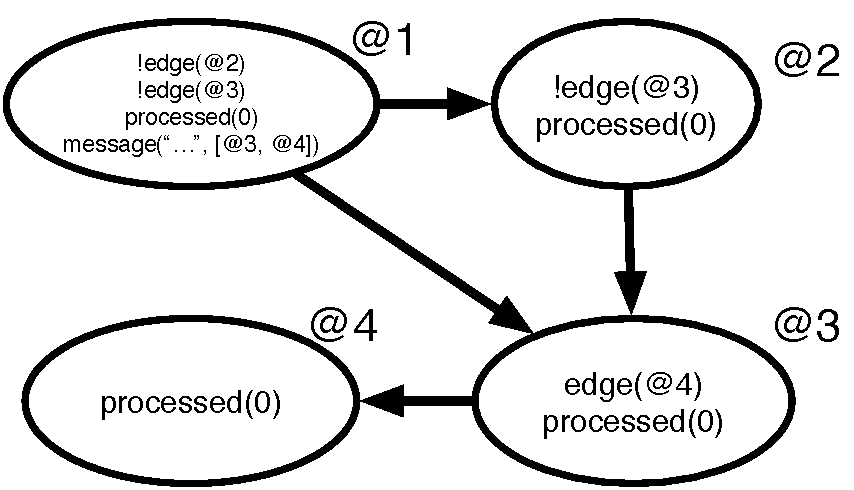
\includegraphics[width=\textwidth]{figures/message/message_trace1}
                \mycap{Initial database.}
                \label{fig:message_trace1}
        \end{subfigure}%
        ~
        \begin{subfigure}[b]{\visitsize\textwidth}
                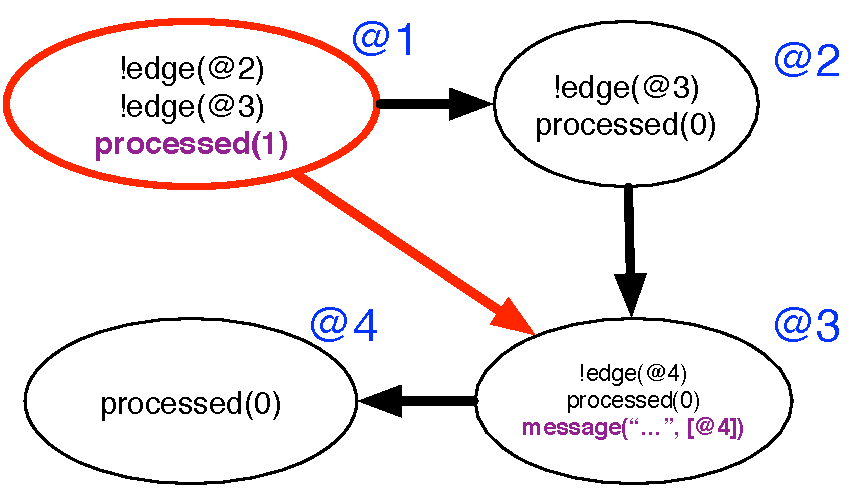
\includegraphics[width=\textwidth]{figures/message/message_trace2}
                \mycap{After applying rule 1 at node \code{@1}.}
                \label{fig:message_trace2}
        \end{subfigure}\\
        \begin{subfigure}[b]{\visitsize\textwidth}
                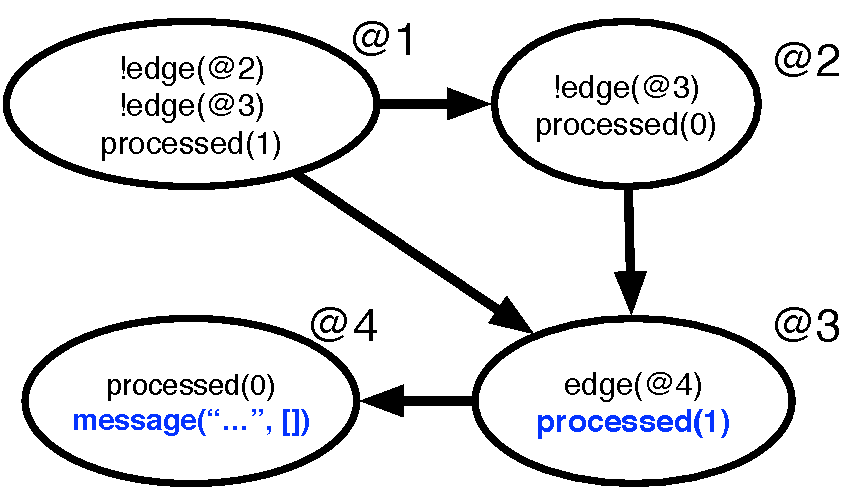
\includegraphics[width=\textwidth]{figures/message/message_trace3}
                \mycap{After applying rule 1 at node \code{@3}.}
                \label{fig:message_trace3}
        \end{subfigure}%
        ~
        \begin{subfigure}[b]{\visitsize\textwidth}
                  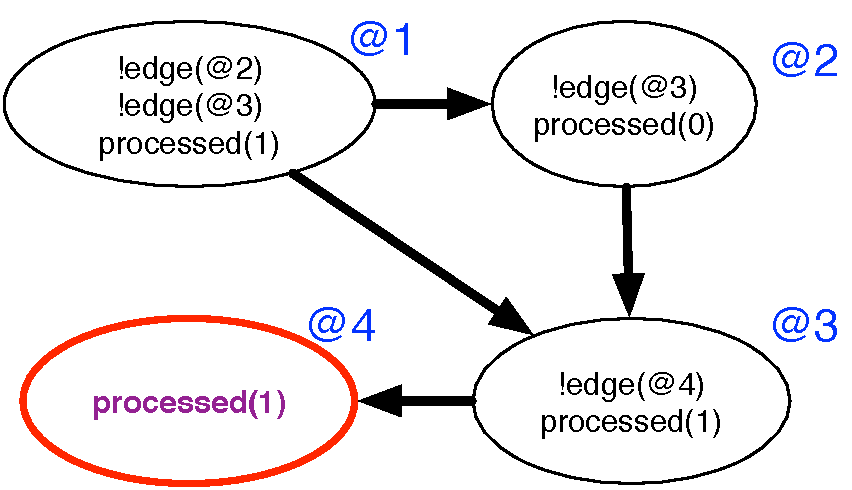
\includegraphics[width=\textwidth]{figures/message/message_trace4}
                  \mycap{After applying rule 2 at node \code{@4}.}
                  \label{fig:message_trace4}
          \end{subfigure}
        \mycap{An execution trace for the message routing program. The message "hello
        world" travels from node \code{@1} to node \code{@4}.}\label{fig:message_trace}
\end{figure}

The attentive reader will wonder how much concurrency is available in this
particular routing implementation. For a single message, there is no concurrency
because the message follows a pre-determined path as it travels from node to
node. However, concurrency arises when the program needs to route multiple
messages. The amount of concurrency is then dependent on the messages routing
lists being non-overlapping. If messages travel in different paths, then there
is more concurrency because more nodes are routing messages at the same time.
